\documentclass{beamer}

\usepackage{xspace}
\usepackage{default}
\usepackage{tikz}
\usepackage{pgfplots}
\usepackage{tabularx}
\usepackage{listings}
\usepackage{booktabs}
\usepackage{etex}
\usepackage{courier}
\usepackage{subfigure}
\usepackage{booktabs}


\lstset{language=Python,
        basicstyle=\footnotesize\ttfamily, % Standardschrift
        breaklines=true,                   % Zeilen werden Umgebrochen
}


\title[IMSI Catcher Detection System]{The IMSI Catcher Detection System\\\small{Final Presentation}}
\author[Thomas Mayer]{Thomas Mayer\\[3mm]\footnotesize {Advisors: Prof.\ Dr.\ Gerhard Schneider}\\\footnotesize{\hspace{-5mm}Dennis Wehrle}\\\footnotesize{\hspace{-6mm}Konrad Meier}}
\institute[Uni Freiburg]{Albert-Ludwigs-Universit\"at Freiburg \\ Technische Fakult\"at \\ Institut f\"ur Informatik \\ Lehrstuhl f\"ur Kommunikationssysteme}
\date{30.\,07.\,2012}

\mode<presentation>{
  \useoutertheme[width=0pt]{zusatz}
  \usetheme{Frankfurt}
	\setbeamertemplate{section in toc shaded}[default][40]
	\setbeamertemplate{subsection in toc shaded}[default][40]
}

\newcommand{\tocsection}[1]{
  \section{#1}
  \begin{frame}{Content}
    \tableofcontents[sectionstyle=show/shaded, subsectionstyle=hide/hide/hide]%show/shaded]%,subsectionstyle=show/show/hide]
  \end{frame}
 }

\begin{document}

\begin{frame}[empty]{}
\maketitle
\end{frame}

\begin{frame}{Content}
\tableofcontents[sectionstyle=show/show,subsectionstyle=show/show/hide]
\end{frame}

\section{Background}
\subsection{IMSI Catcher}
\begin{frame}{Mode of Operation}
\begin{center}
	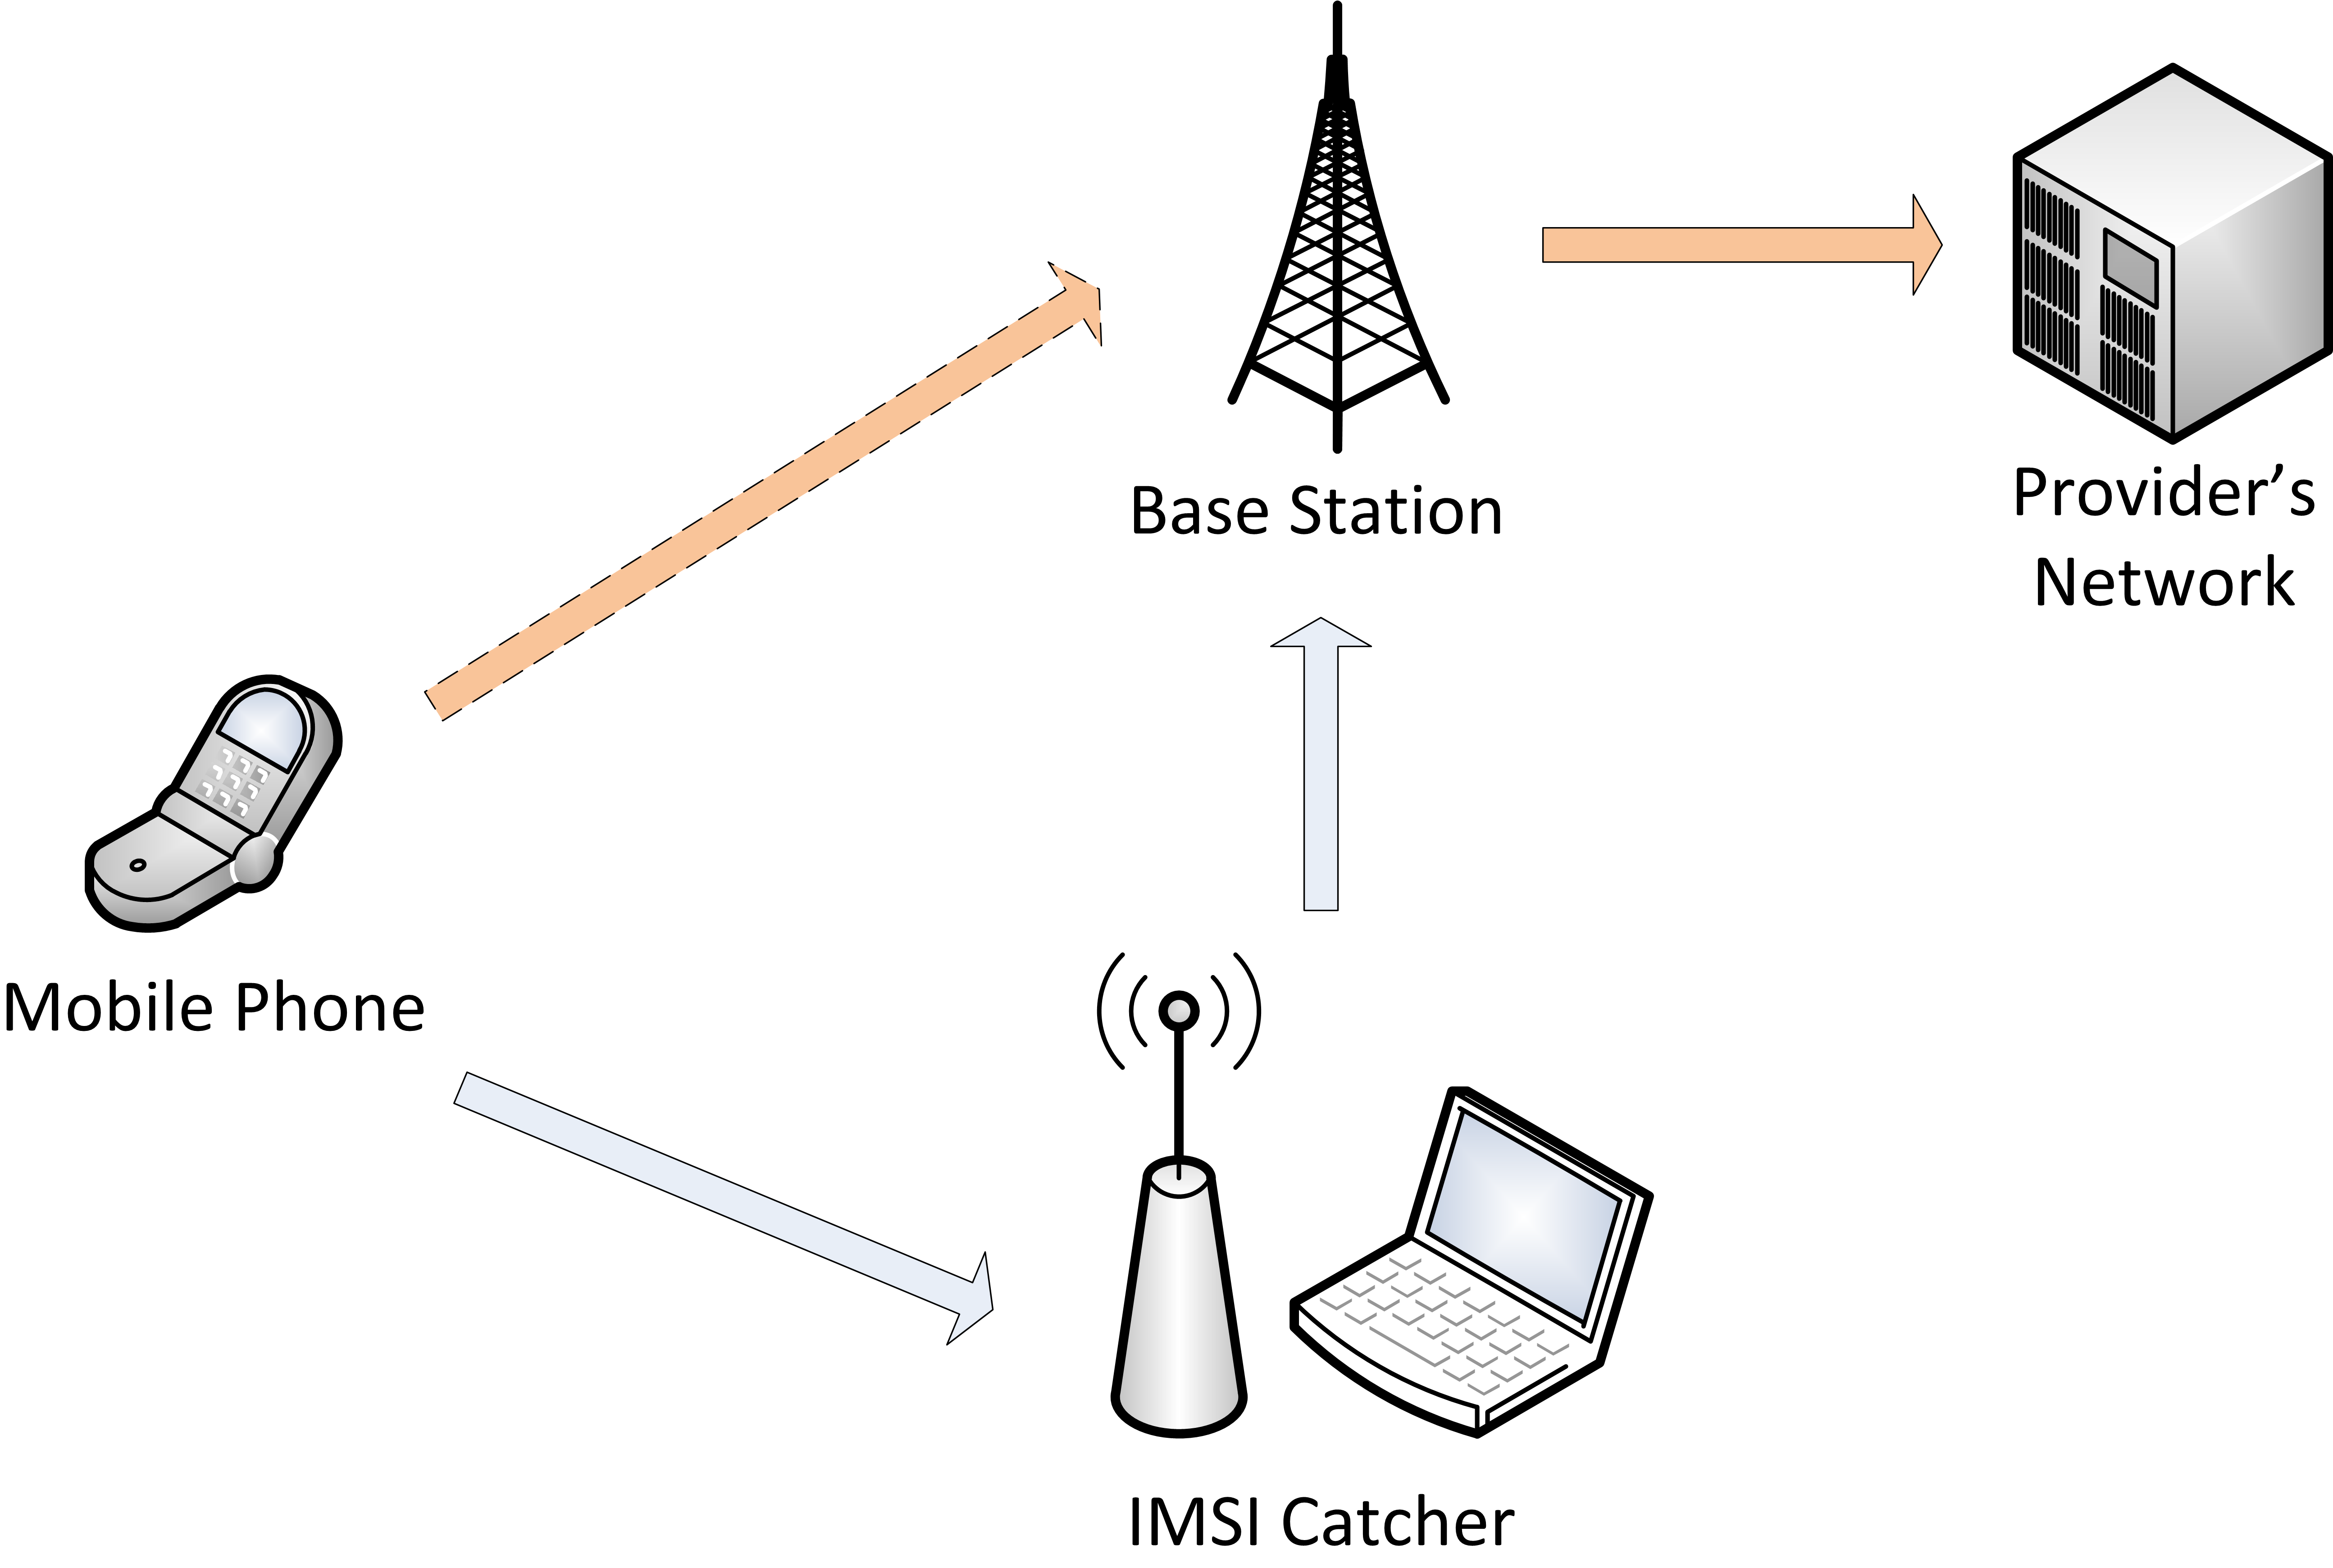
\includegraphics[width=.9\textwidth]{IMSICatcher}
\end{center}
\end{frame}

\begin{frame}{Threats}
\begin{block}{Technical Possibilities}
\begin{itemize}
	\item Extraction of IMSI and IMEI
	\item Tapping and recording of phone calls
	\item Localisation of subscribers
	\item Suppression of communication
\end{itemize}
\end{block}
Main concerns:
\begin{itemize}
	\item Hard to prove operation in retrospect
	\item \textcolor{red}{Private abuse (eavesdropping/industrial espionage)}
	\item Procedural law situation
\end{itemize}
... risk intensified by homebrew IMSI catcher projects!
\end{frame}

\subsection{IMSI Catcher Detection}
\begin{frame}{Detection}
Main Question: How to detect such a device?
\begin{itemize}
	\item<1-> Actively connect to the catcher
	\begin{itemize}
		\item<1-> Localisation possible once connected
		\item<1-> IMSI and IMEI already given up
	\end{itemize}
	\item<1-> \color<2>{red}Passively gather information
\end{itemize}
\vspace{.8cm}
\visible<2>{Procedure: Information that is publicly available
\begin{itemize}
	\item Broadcast Control Channel
	\begin{itemize}
		\item System Information Messages 1-4
		\item System Information 2 and 3 are of special interest
	\end{itemize}
	\item Paging Channel
	\item Parameters that can be measured
\end{itemize}
}
\end{frame}

\begin{frame}{Parameters}{Basic Information}
Parameters for identification harvested from System Information:
\begin{itemize}
	\item ARFCN
	\item Country and Provider Codes
	\item Cell ID and Location Area Code
	\item Neighbouring Cell List
\end{itemize}
\begin{alertblock}<2>{Main Problem}
Parameters that can be set, can be forged!
\end{alertblock}
\end{frame}

\begin{frame}{Parameters}{Additional Information}
Paramteres that are measured:
\begin{itemize}
    \item Signal Strength
\end{itemize}
PCH Parameters:
\begin{itemize}
    \item Paging Messages
    \item Immediate Assignments
\end{itemize}
Databases:
\begin{itemize}
    \item Track parameters over time for changes
    \item Compare parameters to static databases (online/offline)
\end{itemize}
\end{frame}

\tocsection{The IMSI Catcher Detection System}
\subsection{Architecture}
\begin{frame}{Overview}
\begin{center}
	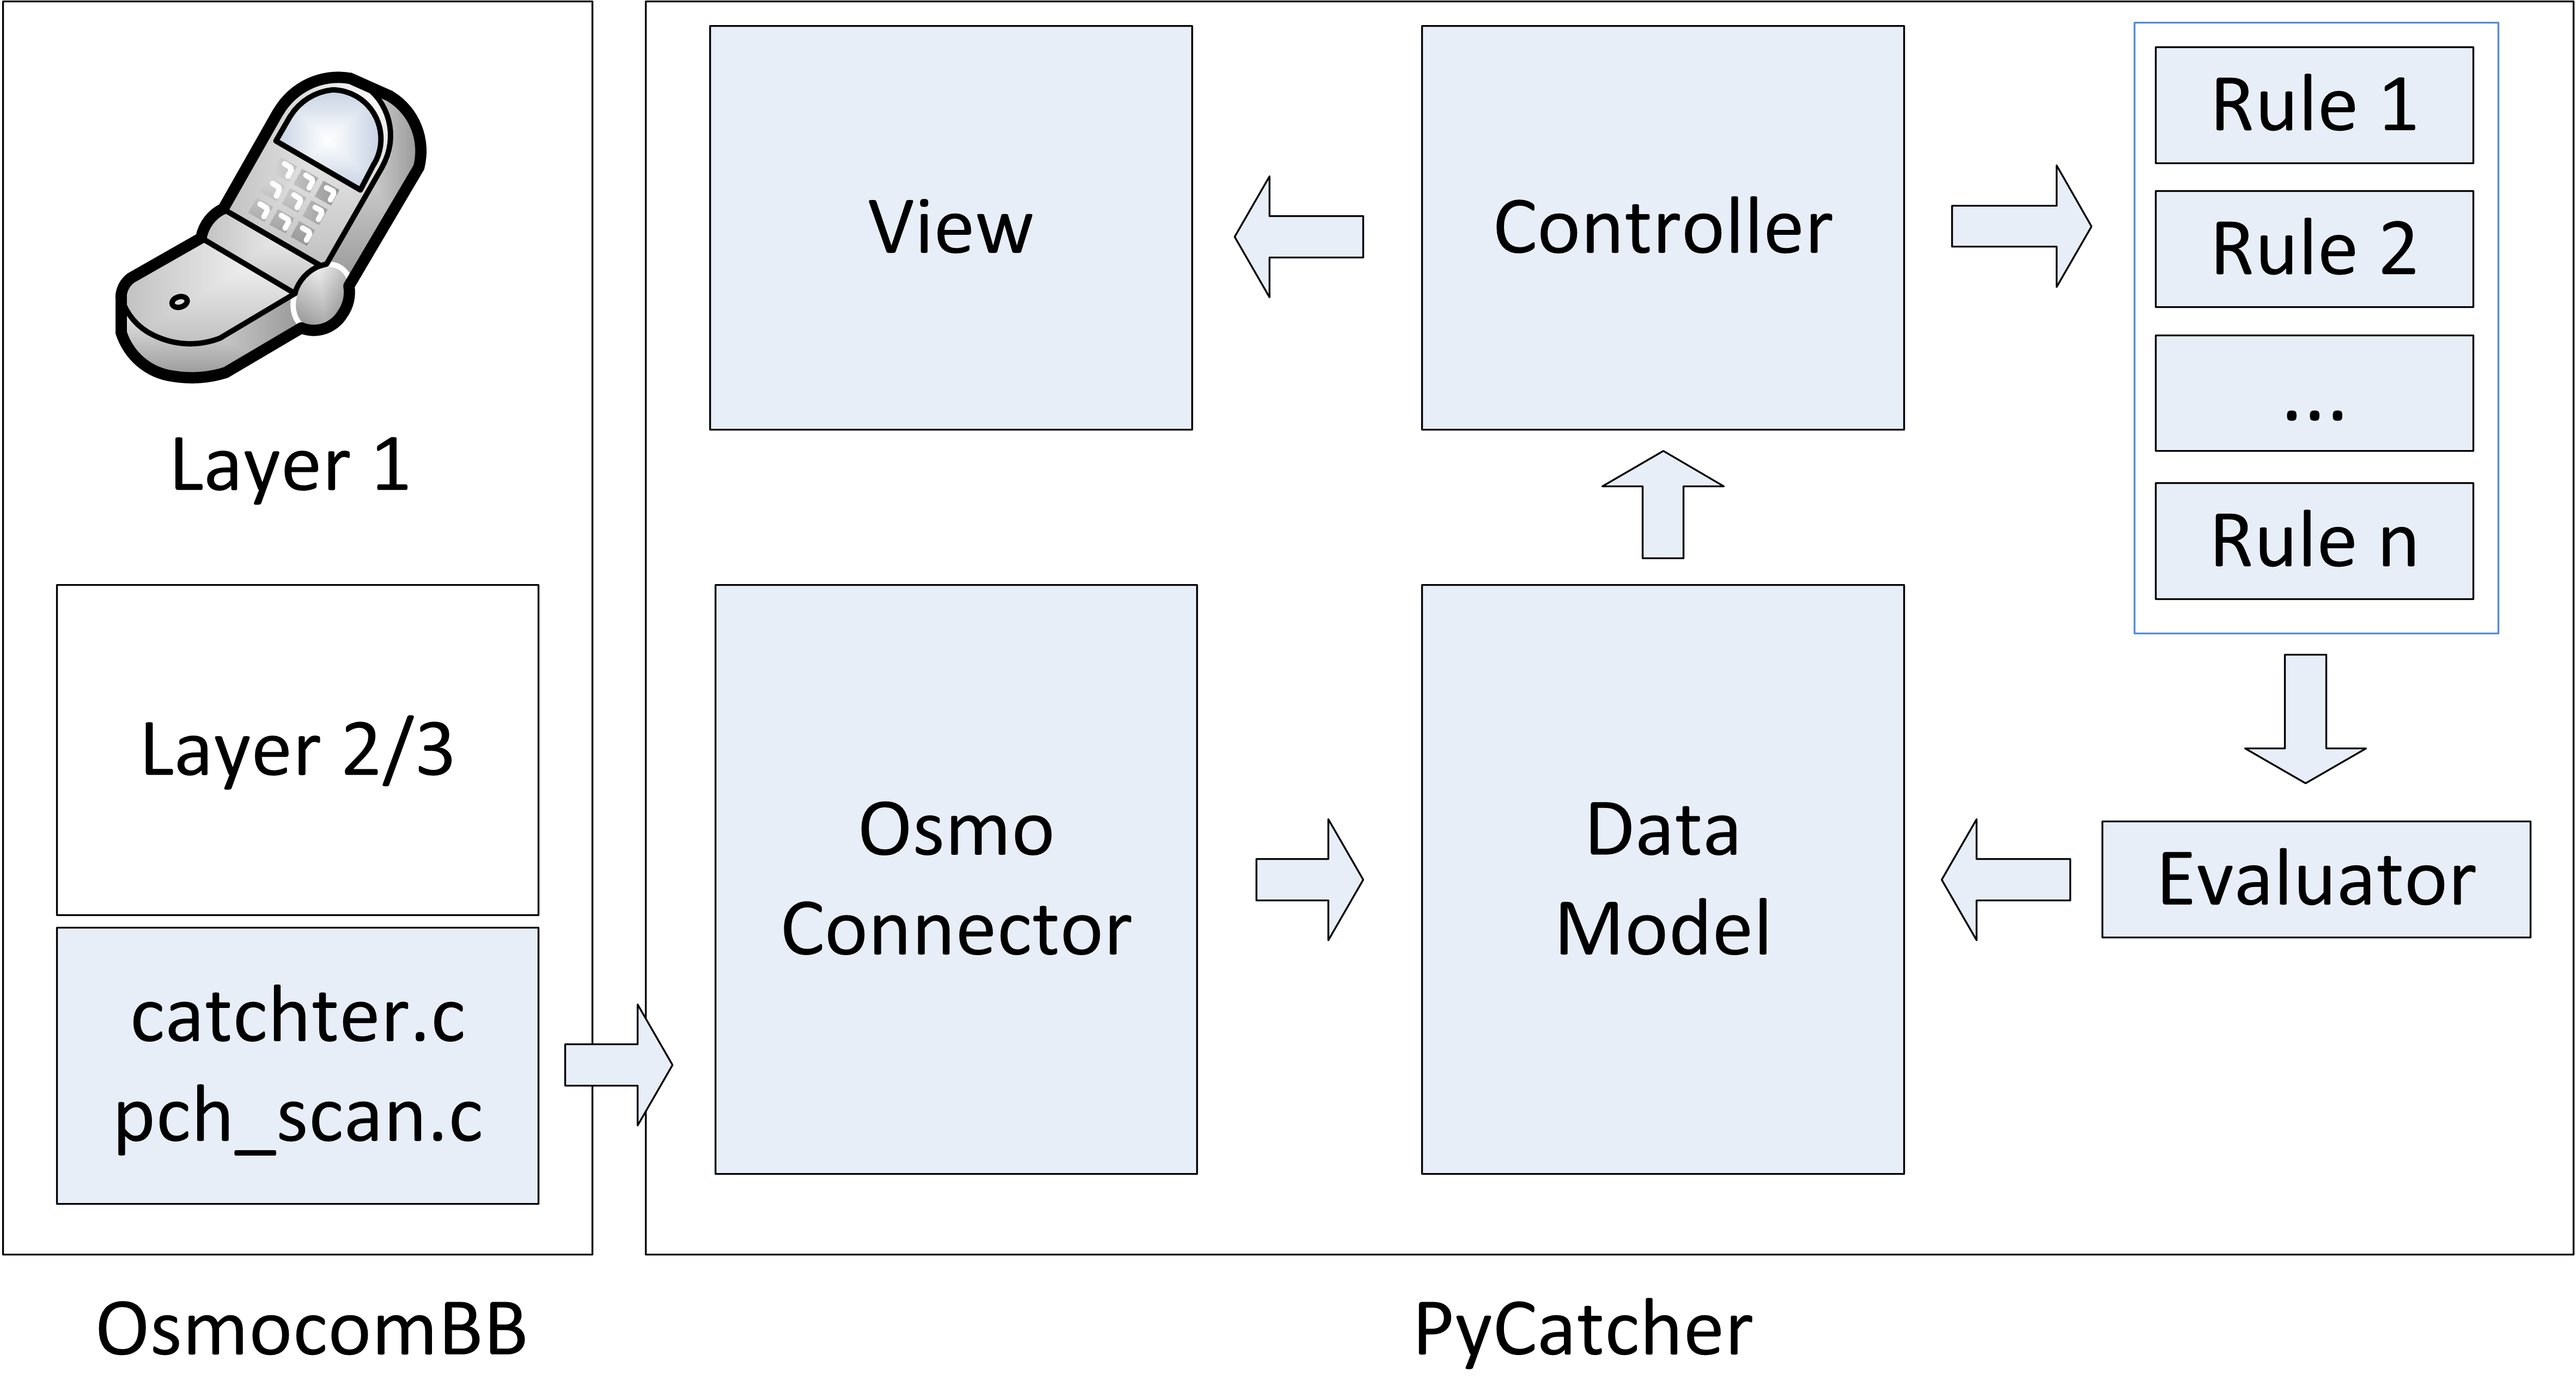
\includegraphics[width=\textwidth]{Architecture_software}
\end{center}
\end{frame}

\subsection{Rules}
\begin{frame}{Rules}{Configuration Rules}
Rules to check parameter integrity:
\begin{itemize}
    \item Country/Provider Mapping
    \item ARFCN/Provider Mapping 
    \item LAC/Provider Mapping
\end{itemize}
\begin{exampleblock}{ARFCN/Provider Mapping}
Checks whether the ARFCN is registered to the Provider:
\begin{itemize}
    \item E-Plus: 975-999, 777-863
    \item T-Mobile: 13-49, 81-102, 122-124, 587-611
    \item Vodafone: 1-12, 50-80, 103-121, 725-751 
    \item O2: 1000-1023, 637-723
\end{itemize}
\end{exampleblock}
\end{frame}

\begin{frame}{Rules}{Context Rules}
Check how well a station fits in its neighbourhood:
\begin{itemize}
    \item Pure Neighbourhoods
    \item Neighbouhood Structure
    \item Cell ID Uniqueness
\end{itemize}
\begin{exampleblock}{Neighbourhood Structure}
Analyses the neighbourhood graph for certain structures:
\begin{itemize}
    \item Nodes with no outgoing/ingoing edges
    \item At least one neighbour needs to be discovered
\end{itemize}
\end{exampleblock}
\end{frame}

\begin{frame}{Rules}{Neighbourhood Structure}
\begin{figure}
\centering
\subfigure[Normal neighbourhood]{
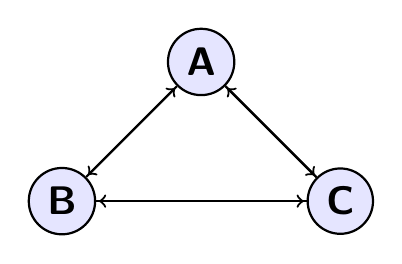
\begin{tikzpicture}[->,shorten >=1pt,auto,node distance=2.5cm,
  thick,main node/.style={circle,fill=blue!10,draw,font=\sffamily\Large\bfseries}]

  \node[main node] (1) {A};
  \node[main node] (2) [below left of=1] {B};
  \node[main node] (3) [below right of=1] {C};

  \path[every node/.style={font=\sffamily\small}]
    (1) edge  node {} (2)
        edge  node {} (3)
    (2) edge  node {} (1)
    	edge  node {} (3)
    (3) edge  node {} (1)
    	edge  node {} (2);
\end{tikzpicture}
}
\subfigure[Tainted neighbourhood]{
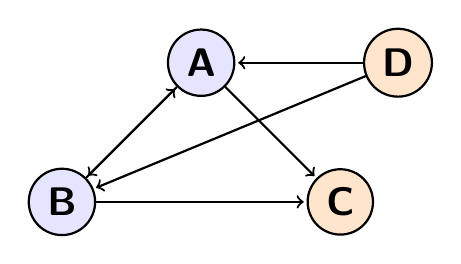
\begin{tikzpicture}[->,shorten >=1pt,auto,node distance=2.5cm,
  thick,main node/.style={circle,fill=blue!10,draw,font=\sffamily\Large\bfseries}]

  \node[main node] (1) {A};
  \node[main node] (2) [below left of=1] {B};
  \node[main node, fill=orange!20] (3) [below right of=1] {C};
  \node[main node, fill=orange!20] (4) [right of=1] {D};

  \path[every node/.style={font=\sffamily\small}]
    (1) edge  node {} (2)
        edge  node {} (3)
    (2) edge  node {} (1)
    	edge  node {} (3)
    (4) edge  node {} (1)
    	edge  node {} (2);
\end{tikzpicture}
}
\end{figure}

\end{frame}

\begin{frame}{Rules}{Database Rules}
Compare parameters against databases:
\begin{itemize}
    \item Cell ID Database
    \item Local Area Database
\end{itemize}
\begin{exampleblock}{Local Area Database}
Uses a database of the area surrounding the ICDS:
\begin{itemize}
    \item Look out for changes in the LAC
    \item Look out for changes in the reception strengths
    \item Tracks Cell IDs for offline use
\end{itemize}
\end{exampleblock}
\end{frame}

\begin{frame}{Rules}{Scan Rules}
Basically the same idea as Local Area Database Rule on a scan-to-scan basis:
\begin{itemize}
    \item Rx Change
    \item LAC Change
\end{itemize}
\end{frame}

\subsection{PCH Scan}
\begin{frame}{PCH Scan}
Why an additional method?
\begin{itemize}
    \item Perfectly configured IMSI Catcher
\end{itemize}
\vspace{.8cm}
IMSI Catcher is only a proxy for a BTS:
\begin{itemize}
    \item Does not get incomming calls for the connected phones
    \item No Paging Messages
    \item Immediate Assignments only if other subscribers are connected
\end{itemize}
Harvest this information and compare it to base levels.
\end{frame}

\tocsection{Results}
\subsection{Results}
\begin{frame}{Results}{Tests}
Test scenarios:
\begin{itemize}
    \item Isolated tests for the single rules
    \item Long term test
    \item Realistic attack scenarios
\end{itemize}
IMSI Catcher was detected whenever it was operating\\
\vspace{.5cm}
Drawbacks:
\begin{itemize}
    \item Can take up to seven minutes for a complete sweep scan
    \item System relies on local information being present
    \item PCH scan is not 100\% reliable, IMSI Catcher could fake Paging Messages
\end{itemize}
\end{frame}

\begin{frame}{Results}{Rule Toughness}
\vspace{-.6cm}
\begin{center}
\begin{tabular}{lll}
\toprule
Rule/Category		&Toughness	    &Limitations\\
\midrule
Configuration Rules	&Easy		    &Correct configuration\\
\midrule
Context Rules		&Medium		    &Consider surroundings\\
Neighbourhood Structure	&Medium		    &Reduce attack types\\
			&		    &and efficiency\\
\midrule
Database Rules		&Hard		    &Reduce attack types\\
Rx Change		&Very Hard	    &Exact transmission power\\
			&		    &and location\\
LAC Change		&Easy		    &Mobile phone not\\
			&		    &announcing itself\\
\midrule
PCH Scan		&Hard		    &Need to fake pagings\\
\bottomrule
\end{tabular}
\end{center}
\end{frame}

\subsection{Future Work}
\begin{frame}{Future Work}
Enhancements:
\begin{itemize}
    \item Filters for sweep scan
    \item Incremental sweep scan
\end{itemize}
New Functionality:
\begin{itemize}
    \item Follow Immediate Assignments on the dedicated channel to reveal if encryption is used
    \item More Rules
    \begin{itemize}
	\item Encryption Rule
	\item GPS location probability Rule
    \end{itemize}
\end{itemize}
\end{frame}

\tocsection{Demo}
\begin{frame}{Demo}
    \centering
    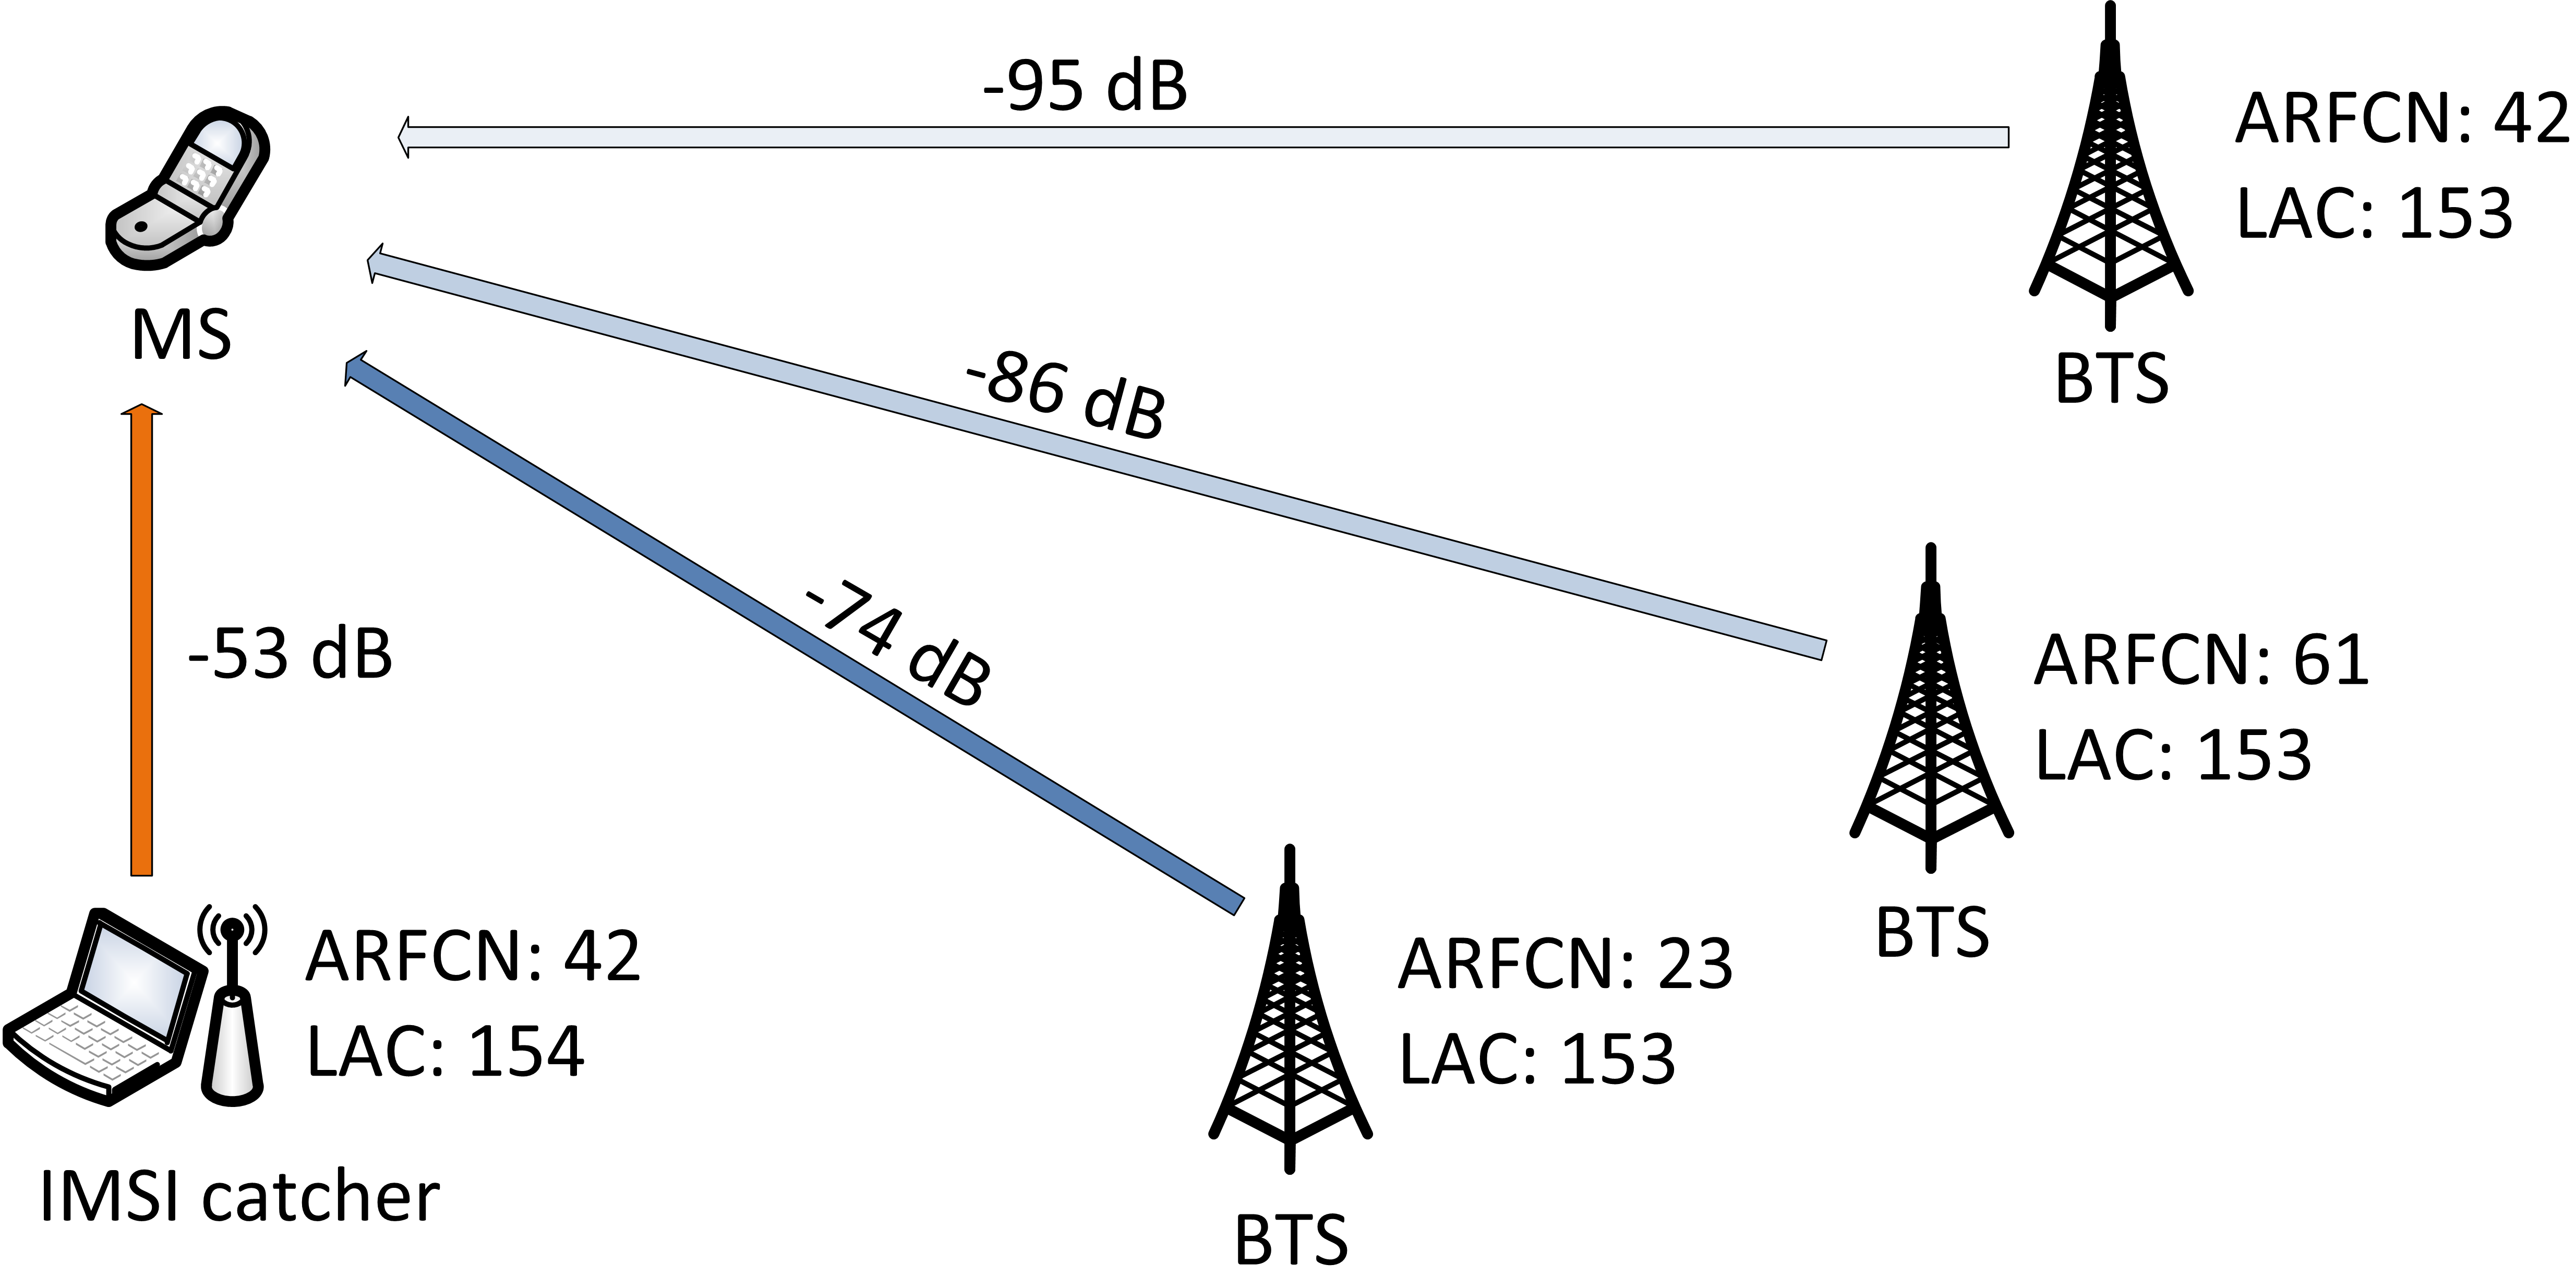
\includegraphics[width=\textwidth]{replace_attack}
\end{frame}

\begin{frame}
\begin{center}
\huge{Thank you for your attention.\\Question?}
\end{center}
\end{frame}
\end{document}

